% Generated from extras.typ. Typst is authoritative; regeneration overwrites this file.
\documentclass{qlnotes-export}

\title{MATH 597: Measure Theory --- Supplementary Material}
\subtitle{Homework 0, problem-solving lectures, and practice problems}
\author{Qiulin Fan}
\date{Winter 2025}

\begin{document}
\mainmatter
\chapter{hw 0}\label{hw-0}

(Not graded.) Read Sections 0.1-0.3 and 0.5-0.6 in Folland's book. Note: I expect you to have seen much but not necessarily all of this material in earlier courses. It is not necessary to know everything by heart right now. However, in order to succeed in the class, you need to be able to read mathematical material at this level of abstraction and (lack of) detail.

\section{Approaching 597}\label{approaching-597}

Let \(A\) be an infinite (not necessarily countable) set, and \(f:A\rightarrow{\mathbb{R}}\) a function. Suppose that for every integer \(N \geq 1\) there exist finite subsets \(A_{N}^{+} \subset A\) and \(A_{N}^{-} \subset A\) such that:

\begin{itemize}
\item
  (i) \(\left. |f(\alpha) \middle| \leq N^{- 1} \right.\) for all \(\alpha \in A\backslash(A_{N}^{+} \cup A_{N}^{-})\);
\item
  (ii) \(\sum_{\alpha \in A_{N}^{+}}f(\alpha) \geq N\);
\item
  (iii) \(\sum_{\alpha \in A_{N}^{-}}f(\alpha) \leq - N\).
\end{itemize}

Prove that for any \(N \geq 1\), there exists a finite subset \(B_{N} \subset A\) such that

\[\left| {597 - \sum\limits_{\alpha \in B_{N}}f(\alpha)} \right| \leq \frac{1}{N}.\]

\begin{proof}

We first take \(A_{N} = A_{N}^{+}\bigcup A_{N}^{-} \subset A\) s.t. \(\left. |f(\alpha) \middle| \leq N^{- 1} \right.\) for all \(\alpha \in A\backslash A_{N}\), as given by the conditions.\\
Now we define \(pos(A_{N}) := \left\{ {\alpha \in A_{N} \mid f(\alpha) \geq 0} \right\}\) and \(neg(A_{N}) := \left\{ {\alpha \in A_{N} \mid f(\alpha) < 0} \right\}\).\\
Let \(gap := \sum_{\alpha \in A_{N}}f(\alpha) - 597\). This is a real number since \(A_{N}\) is finite.\\
\strut \\
Case 1: if \(gap < 0\), then we need to fill in more elements whose image under \(f\) sum up to be positive to make the sum close to 597 from below.\\
We then take a finite set \(B_{N}^{+} \subset A\) s.t. \(\sum_{\alpha \in B_{N}^{+}}f(\alpha) \geq \lceil - gap + \sum_{\alpha \in pos(A_{N})}f(\alpha)\rceil\).\\
Since \(B_{N}^{+}\bigcap A_{N} \subset A_{N}\), we have

\[\sum\limits_{\alpha \in B_{N}^{+}\bigcap A_{N}}f(\alpha) \leq \sum\limits_{\alpha \in pos(A_{N})}f(\alpha)\]

and since \(B_{N}^{+} = (B_{N}^{+}\backslash A_{N})\coprod(B_{N}^{+}\bigcap A_{N})\), we have

\[\sum\limits_{\alpha \in B_{N}^{+}}f(\alpha) = \sum\limits_{\alpha \in B_{N}^{+}\backslash A_{N}}f(\alpha) + \sum\limits_{\alpha \in B_{N}^{+}\bigcap A_{N}}f(\alpha)\]

By (1) and (2), it is clear that

\[\sum\limits_{\alpha \in B_{N}^{+}\backslash A_{N}}f(\alpha) \geq - gap\]

(3) means that the elements in \(B_{N}^{+}\backslash A_{N}\) have big enough image sum to fill the gap. And by definition, for all \(\alpha \in B_{N}^{+}\backslash A_{N}\), we have \(\left. |f(\alpha) \middle| \leq \frac{1}{N} \right.\). This means that each element in this finite \(B_{N}^{+}\backslash A_{N}\) takes up only a small portion of the sum, bounded by \(1/N\). Together with (3), it follows that there is some subset \(B_{N}' \subset B_{N}^{+}\backslash A_{N}\) s.t. \(\sum_{\alpha \in B_{N}'}f(\alpha) \in \lbrack - gap - 1/N, - gap + 1/N\rbrack\). So for the finite set \(A_{N}\bigcup B_{N}'\), we have

\[\sum\limits_{\alpha \in A_{N}\bigcup B_{N}'}f(\alpha) = \sum\limits_{\alpha \in A_{N}}f(\alpha) + \sum\limits_{\alpha \in B_{N}'}f(\alpha) \in \lbrack 597 - 1/N,597 + 1/N\rbrack\]

\begin{center}

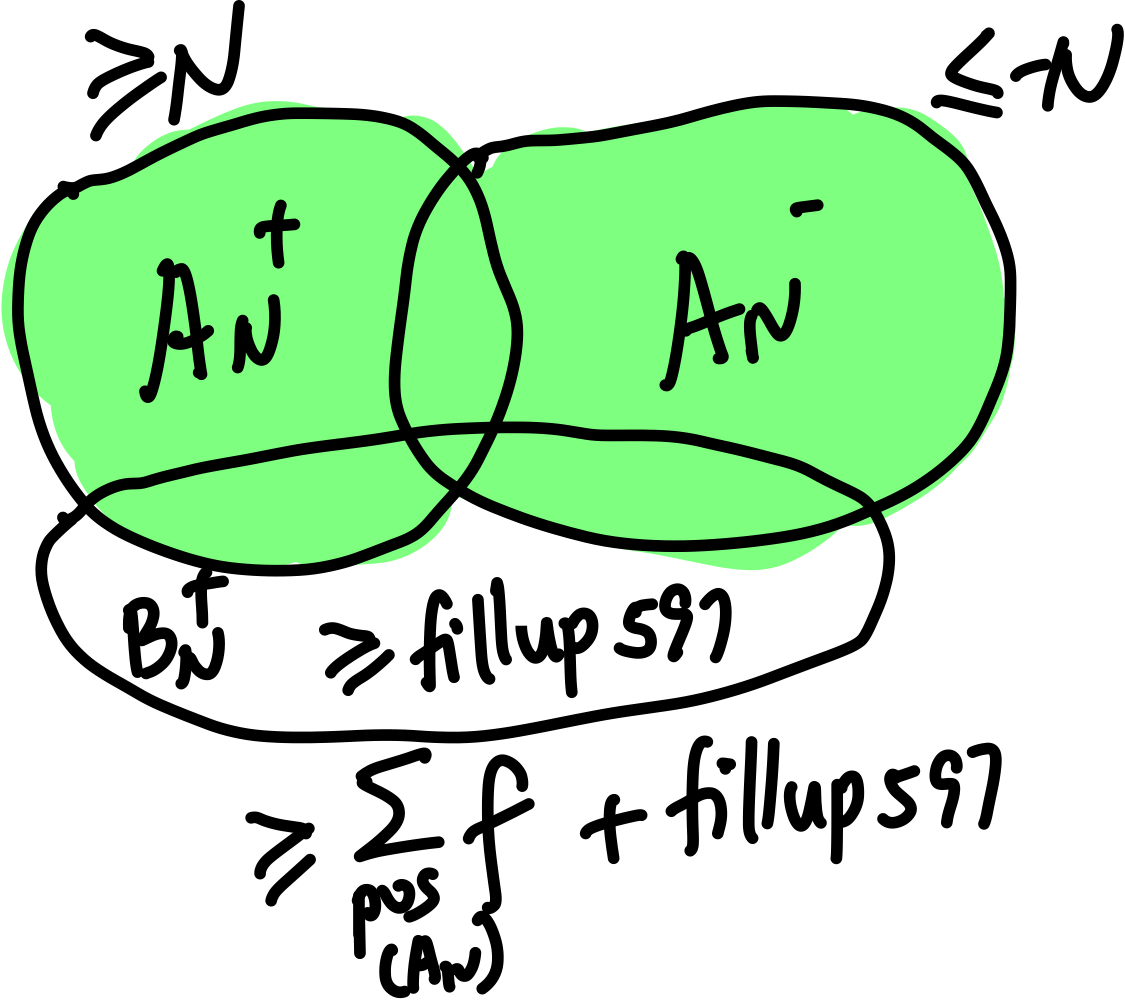
\includegraphics[width=0.3\linewidth,height=\textheight,keepaspectratio]{assets/extras--figure-raster-001.png}

\end{center}

Case 2: if \(gap > 0\), then we need to fill in more elements whose image under \(f\) sum up to be negative to make the sum close to 597 from above.\\
We then take finite \(B_{N}^{-} \subset A\) s.t. \(\sum_{\alpha \in B_{N}^{-}}f(\alpha) \leq \lfloor - gap + \sum_{\alpha \in neg(A_{N})}f(\alpha)\rceil\).\\
For the same reason as case 1, we get

\[\sum\limits_{\alpha \in B_{N}^{-}\backslash A_{N}}f(\alpha) \leq - gap\]

And by definition, for all \(\alpha \in B_{N}^{-}\backslash A_{N}\), we have \(\left. |f(\alpha) \middle| \leq \frac{1}{N} \right.\). Together with (5), it follows that there is some subset \(B_{N}' \subset B_{N}^{-}\backslash A_{N}\) s.t. \(\sum_{\alpha \in B_{N}'}f(\alpha) \in \lbrack - gap - 1/N, - gap + 1/N\rbrack\). So for the finite set \(A_{N}\bigcup B_{N}'\), we have

\[\sum\limits_{\alpha \in A_{N}\bigcup B_{N}'}f(\alpha) = \sum\limits_{\alpha \in A_{N}}f(\alpha) + \sum\limits_{\alpha \in B_{N}'}f(\alpha) \in \lbrack 597 - 1/N,597 + 1/N\rbrack\]

\hfill\break
Case 3: \(gap = 0\), then we are done.\\
This finishes the proof of the statement.

\end{proof}

\begin{qlremark}{Remark}

意思是说 \(f\) 对于任意小的 bound 都存在一个 infinite set 上能够限于这一 bound 内(可逼近 0), 而在一个 finite set 上总和可以任意大. 要证明的是对于任意一个数, 我们都可以指定一个 finite set, 让这个函数在这个 finite set 上的总和无限接近这个数. 这里以 597 为例. 对于这个 bounded 的 infinite set, 我们简称它为 big flat set, 其补集称之为 small wavy set.\\
\strut \\
这题思考甚久. 一开始卡住的原因就是局限于这个 big flat set 的 sum postive 和 sum negative 这两个划分上, 因为这占了条件中很大一部分笔墨. 但是最后却发现实际上这个集合在第一步构造中并没有用, 甚至作用一直都不大, 只用一边即可. 并且, 这两个条件不仅是透明条件, 而且我们甚至应该构建自己的 "all positive" 和 "all negative" set.\\
\strut \\
为什么说这个 sum postive 和 sum negative 划分几乎没用: 因为它基本不给出任何 invariant 的信息. 举例: sum postive set 的 image sum \(\geq 100\), sum negative set 的 image sum \(\leq - 100\), 它们交的部分, 其可能的 image sum 上下都可以 unboundly large, 可以是 99999, 唯一能 imply 的信息是两边 \(A_{N} + \backslash A_{N}^{-}\) 和 \(A_{N} - \backslash A_{N}^{+}\) 之间的差距大于等于 200, 但是这也没用, 因为我们对元素个数也没有 control over.因而我们想要准确地逼近一个数, 必须要靠外界的大小全都 singly bounded 的元素.\\
\strut \\
于是关键的解题点在于: small wavy set 的有限性, 所以我们可以把它的值设做 \(gap\), 并可以把它分为全正和全负的两个 portion. 这样的目的是: 我们等于给 \(\mathcal{P}(A)\) 中每个集合赋予了一个 measure, 等于 image sum under \(f\), 而局限在 small wavy set 上, 这个 measure 最小的集合就是 all negative set, 最大的集合就是 all positive set. 从而, 我们先比较 \(gap\) 和 597 的大小, 根据其正负, 制定一个 (差值 \(\pm\) allPos/Neg set 的 function measure) 的 bound, 并创造第二个 big wavy set \(B_{N}\). 这个 \(B_{N}\) 和 \(A_{N}\) 可能相交, 但是这一次, 我们可以 control over \(B_{N}\backslash A_{N}\) 的部分, 因为这部分的值必须大于 \(gap\) 和 597 的差值, 并且这个部分还属于 \(A_{N}\) 外的 big flat set, 其中每个元素的函数值都是 bounded by a small number 的.

\end{qlremark}

\section{Limsup and Liminf}\label{limsup-and-liminf}

Let \(X\) be a nonempty set, and \(A,B\) subsets of \(X\). Define a sequence \((E_{n})_{n = 1}^{\infty}\) of subsets of \(X\) by

\[E_{n} = \left\{ \begin{matrix}
{A\ } & {\text{if}\ n\ \text{is a prime number,}} \\
{B\ } & \text{otherwise.}
\end{matrix} \right.\]

Characterize the sets \(\operatorname{lim\, sup}E_{n}\) and \(\operatorname{lim\, inf}E_{n}\) (see §0.1 in Folland for notation).

\begin{qlsolution}{Solution}

By definition,

\[\operatorname{lim\, sup}(E_{n}) = \bigcap\limits_{k = 1}^{\infty}\bigcup\limits_{n = k}^{\infty}E_{n}\]

For each \(k \in {\mathbb{N}}\), there are infinitely many \(n \geq k\) such that \(n\) is prime, and also there are infinitely many \(n \geq k\) such that \(n\) is not prime. So \(\bigcup_{n = k}^{\infty}E_{n} = A\bigcup B\). Therefore

\[\operatorname{lim\, sup}(E_{n}) = \bigcap\limits_{k = 1}^{\infty}(A\bigcup B) = A\bigcup B\]

By definition,

\[\operatorname{lim\, inf}(E_{n}) = \bigcup\limits_{k = 1}^{\infty}\bigcap\limits_{n = k}^{\infty}E_{n}\]

For each \(k \in {\mathbb{N}}\), there are infinitely many \(n \geq k\) such that \(n\) is prime, and also there are infinitely many \(n \geq k\) such that \(n\) is not prime. So \(\bigcap_{n = k}^{\infty}E_{n} = A\bigcap B\). Therefore

\[\operatorname{lim\, inf}(E_{n}) = \bigcup\limits_{k = 1}^{\infty}(A\bigcap B) = A\bigcap B\]

\end{qlsolution}

\section{Polynomial Convergence}\label{polynomial-convergence}

Let \(f:{\mathbb{Z}}_{\geq 0} \times {\mathbb{Z}}_{\geq 0}\rightarrow{\mathbb{R}}\) be a function with the property that for every polynomial

\[p(x) = x^{d} + a_{1}x^{d - 1} + \cdots + a_{d}\]

with integer coefficients, we have that

\[\lim\limits_{n\rightarrow\infty}f(n,p(n)) = \lim\limits_{n\rightarrow\infty}f(p(n),n) = 0.\]

Does it follow that \(f(m,n)\rightarrow 0\) as \(m,n\rightarrow\infty\)? In other words, given \(\epsilon > 0\), does there exist \(N \geq 0\) such that \(\left. |f(m,n) \middle| < \epsilon \right.\) whenever \(\left. |m \middle| , \middle| n \middle| \geq N \right.\)? Give a proof or a counterexample.

\begin{qlsolution}{Solution}

Consider this function:

\[\begin{matrix}
{f(m,n) = \{ 1,\text{if}\ m = 2^{n}} \\
{0,\text{otherwise}}
\end{matrix}\]

Let \textbf{\(p\) be arbitrary polynomial with integer coefficients.} Then there must be at most finite \(n\) such that \(p(n) = 2^{n}\). This is guaranteed by the asymptotic behavior of polynomial and exponential function: \(\lim_{n\rightarrow\infty}\frac{p(n)}{2^{n}} = 0\). So there exists some \(N \in {\mathbb{N}}\) s.t. \(\frac{p(n)}{2^{n}} < 1/2\) for all \(n \geq N\), therefore \textbf{\(f(p(n),n)\) is eventually 0}.\\
Also, there must be at most finite \(n\) such that \(2^{p(n)} = n\), i.e. \(p(n) = \log_{2}n\). This is guaranteed by the asymptotic behavior of polynomial and logarithmic function: \(\lim_{n\rightarrow\infty}\frac{\log_{2}n}{p(n)} = 0\). So there exists some \(N \in {\mathbb{N}}\) s.t. \(\frac{\log_{2}n}{p(n)} < 1/2\) for all \(n \geq N\), therefore \textbf{\(f(n,p(n))\) is eventually 0}.\\
This confirms that \(\lim_{n\rightarrow\infty}f(n,p(n)) = \lim_{n\rightarrow\infty}f(p(n),n) = 0\) for any polynomial \(p\) with integer coefficients.\\
Then we consider the sequence \(((2^{n},n))_{n \in {\mathbb{N}}}\). For any \(n \in {\mathbb{N}}\), \(f((2^{n},n)) = 1\), so the sequential limit is \(1\). This completes the counterexample.

\begin{center}

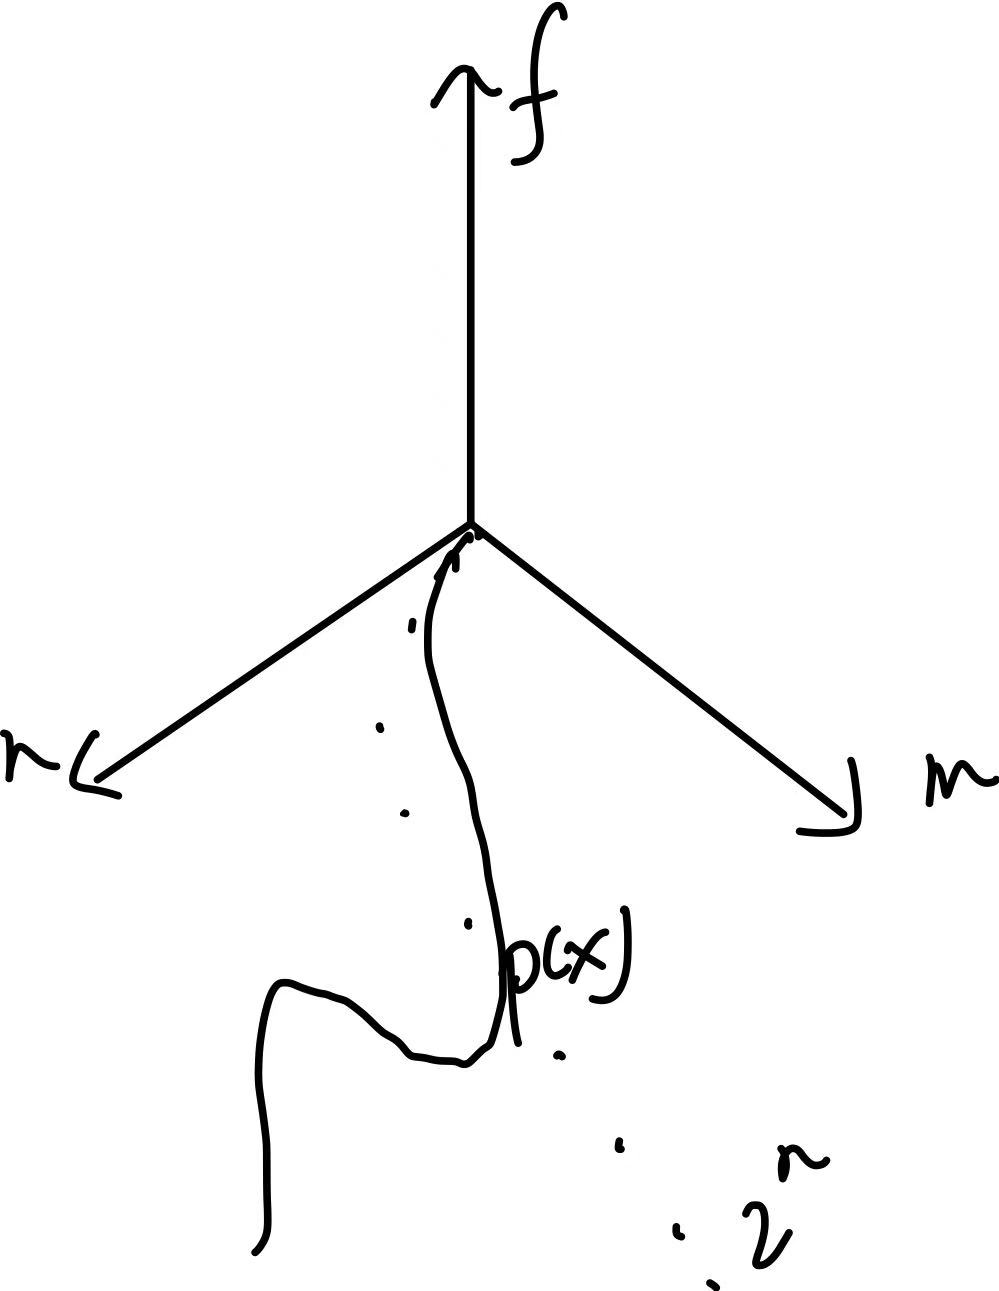
\includegraphics[width=0.3\linewidth,height=\textheight,keepaspectratio]{assets/extras--figure-raster-002.jpg}

\end{center}

\end{qlsolution}

\begin{qlremark}{Remark}

\(f\) 是一个二元 input 的函数, 其满足, 将任何一个 polynomial 函数的 graph input 进入, limit behavior 都会趋近于 0.\\
这个表现乍看很雾. 所以不如试一试: identity polynomial 和 trivial polynomial. 得到 \(\lim_{n\rightarrow\infty}f(1,n) = \lim_{n\rightarrow\infty}f(n,1) = 0\), 以及 \(\lim_{n\rightarrow\infty}f(n,n) = 0\), 以及可想折中的情况: 这两个 input 的增长速度是 polynoimial relation 的情况下(一个是 \(n\), 一个是 \(p(n)\))也是趋近于 0 的, 这个表现像是这个函数在两个 input 各自以任意速度增长时 converge to 0.\\
\strut \\
但是直觉告诉我们这个 polynomial 关系的增长速度不能代表增长速度差距更大的情况, 比如 exponential.遂想到解题点: 这个 limit behavior, 针对的是任意 polynomial, 但是是随意选择一个固定的 polynomial 之后, 才在这个固定的 polynomial 上有这个行为.\\
\strut \\
Then we think about: 一个在 exponential graph as input 上一直得到固定值, 在其他 input 上都得到 0 的函数. 从而对于这个 exponential graph input 的 seq, 函数的 limit behavior 是一个固定值; 而对于任意的 polynomial, 函数的 limit behavior 都是 0，因为任意 polynomial 函数, 和一个 exponential 函数至多有有限个重合点, asymptotic 增长速度不同.\\
\strut \\
(PS: 笔者在思考构造时想到过一个很 silly 的问题: 对于任意两个整数 \(x,y\)，是否都存在一个无常数项的整系数 polynomial 使得 \(p(x) = y\)? 答:很显然不是. 回忆小学数学: 我们只要选择和 \(x\) 没有 common factor 的 \(y\) 即可得反.)

\end{qlremark}
\end{document}
